%%% collusion-attacks.tex: -*- LaTeX -*-  DESCRIPTIVE TEXT.
%%% 
%%% Copyright (c) 2017 Brian J. Fox & Orchid Labs, Inc.
%%% Author: Brian J. Fox (bfox@meshlabs.org)
%%% Author: A truckload of others
%%% Birthdate: Tue Oct 10 12:04:54 2017.
In this section we explore what kinds of information are available to
different nodes for different chain structures and analyze how
different types of collusion impact a user's privacy.

\subsection{Information Available to an Individual Relay or Proxy}
\label{relay-proxy-info-known}

Due to the inherent structure of IP-based networking, and the \Orchid{} protocol, relay nodes gain access to the following information:

\begin{itemize}
\item The IP Addresses of all their connections. This is required to perform IP communication.
\item The size, timing, and number of packets they forward. This is required to perform IP communication.
\item The public key which controls the tokens paying them. This is required for the sale of bandwidth.
\end{itemize}

\subsection{Potential Parties to a Collusion}
\label{sec:collusion}

The following roles can collude to expose customer information:

\begin{itemize}
\item Global Adversary. An attacker with a global view of the network. \Orchid{} does not currently protect against this type of attacker. Untrustworthy with probability 1.
\item ISP. The user's Internet service provider. Untrustworthy with probability $s$.
\item Web. The webserver the proxy is connected to. Untrustworthy with probability $w$.
\item Relay$_n$. The nth relay in the chain. Untrustworthy with probability $\frac{a}{n}$.
\item Proxy. The relay proxying bandwidth for the user. Untrustworthy with probability $\frac{a}{n}$.
\end{itemize}

\subsection{Types of Attack}

The central goal of collusion attacks is the linking of a specific
\Orchid{} customer with a specific SSL connection. There are two ways
this can be done:

\begin{itemize}
\item Relation. When this is possible, the attacker can deduce which
  customer is talking to a given website simply by doing lookups of
  linked IP addresses.
\item Timing. By controlling the timing of packets a link which cannot
  be looked up can be inferred.
\end{itemize}

\subsection{Zero Relays, Zero Proxies: Direct Connection}

Although the \Orchid{} system is not used when a Customer connects
directly to a website, we feel it is important to review what
informational risk are present in this setup.

\begin{center}
\begin{tabular}{l | l | l | l}
  ISP & Website & P(Relate)          & P(Timing) \\
  \hline
  x   &         & $s$                & \\
  \hline
      & x       & $w$                & \\
\end{tabular}
\end{center}

%% \begin{itemize}
%% \item ISP can directly relate Customer traffic. $p = s$
%% \item Website alone can directly relate Website traffic. $p = w$
%% \end{itemize}

In the above table, an ``X'' indicates participation in a collusion,
and the values in P(Relate) and P(Timing) indicates the chance of this
happening. Lines where attacks are not possible are omitted, as are
lines with extraneous ``X''s.

\subsection{Zero Relays, One Proxy}

%% \begin{figure}[htbp]
%%   \centering
%%   \includegraphics[width = 200pt]{sc}
%%   \caption{}
%% \end{figure}

\begin{center}
\begin{tabular}{l | l | l | l | l}
  ISP & Proxy & Website & P(Relate)          & P(Timing) \\
  \hline
      & x     &         & $\frac{a}{n}$      & \\
  \hline
  x   &       & x       &                    & $sw$ \\
\end{tabular}
\end{center}

%% \begin{itemize}
%% \item Proxy can relate Website traffic. $p = \frac{a}{n}$.
%% \item ISP + Website can relate Website traffic. $p = sw$.
%% \end{itemize}

\subsection{One Relay, One Proxy}

%% \begin{figure}[htbp]
%%   \centering
%%   \includegraphics[width = 200pt]{stc}
%%   \caption{}
%% \end{figure}

\begin{center}
\begin{tabular}{l | l | l | l | l | l}
  ISP & Relay$_1$ & Proxy & Website & P(Relate)          & P(Timing) \\
  \hline
      & x         & x     &         & $(\frac{a}{n})^2$  & \\
  \hline
      & x         &       & x       & $w(\frac{a}{n})$   & \\
  \hline
  x   &           & x     &         & $s(\frac{a}{n})$   & \\
  \hline
  x   &           &       & x       &                    & $sw$ \\
\end{tabular}
\end{center}

Note that although it may appear this configuration can support
``bandwidth burning'' on the path running between the Customer and the
Proxy, because the Proxy still controls the timing of, packets no
timing attack is prevented.

%% \begin{itemize}
%% \item Relay$_1$ + Proxy can relate customer traffic. $p = (\frac{a}{n})^2$
%% \item Relay$_1$ + Website can relate Website traffic. $p = w\frac{a}{n}$
%% \item ISP + Proxy can relate all Website traffic. $p = s\frac{a}{n}$
%% \item ISP + Website can timing attack Website traffic. $p = sw$
%% \end{itemize}

\subsection{Two Relays, One Proxy}

%% \begin{figure}[htbp]
%%   \centering
%%   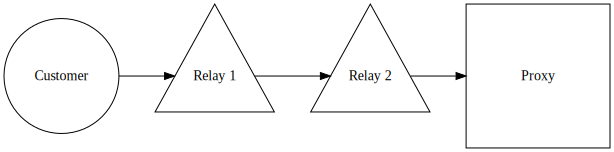
\includegraphics[width = 200pt]{sttc}
%%   \caption{}
%% \end{figure}

\begin{center}
\begin{tabular}{l | l | l | l | l | l | l}
  ISP & Relay$_1$ & Relay$_2$ & Proxy & Website & Relate             & Timing \\
  \hline
      & x         &           & x     &         & $(\frac{a}{n})^2$  & \\
  \hline
  x   &           & x         & x     &         & $s(\frac{a}{n})^2$ & \\
  \hline
      & x         & x         &       & x       & $w(\frac{a}{n})^2$ & \\
  \hline
  x   &           & x         &       & x       & $sw(\frac{a}{n})$  & \\
  \hline
      & x         &           &       & x       &                    & $s(\frac{a}{n})$ \\
  \hline
  x   &           &           &       & x       &                    & $sw$ \\
\end{tabular}
\end{center}


%% \begin{itemize}
%% \item Proxy + Relay$_1$ can relate customer traffic. $p = (\frac{a}{n})^2$
%% \item Proxy + Relay$_2$ + ISP can relate customer traffic. $p = s(\frac{a}{n})^2$
%% \item Website + Relay$_1$ + Relay$_2$ can relate Website traffic. $p = w(\frac{a}{n})^2$
%% \item Website + Relay$_2$ + ISP can relate Website traffic. $p = sw\frac{a}{n}$
%% \item Website + Relay$_1$ can timing attack Website traffic. $p = w\frac{a}{n}$ [can be prevented with bandwidth burning]
%% \item Website + ISP can timing attack Website traffic. $p = sw$ [can be prevented with bandwidth burning]
%% \end{itemize}

%% Total risk without bandwidth burning is therefore: $$(1+w+s)(\frac{a}{n})^2 + (sw+w)\frac{a}{n}$$ and $$(1 + w + s) (\frac{a}{n})^2$$ with bandwidth burning.

Note that this configuration can support ``bandwidth burning'' on the
path running between the Customer and Relay$_2$. If it is employed,
both timing attacks are made more difficult by a factor of
$\frac{a}{n}$.

\subsection{Three Relays, One Proxy}

%% \begin{figure}[htbp]
%%   \centering
%%   \includegraphics[width = 200pt]{stttc}
%%   \caption{}
%% \end{figure}

\begin{center}
\begin{tabular}{l | l | l | l | l | l | l | l}
  ISP & Relay$_1$ & Relay$_2$ & Relay$_3$ & Proxy & Website & Relate             & Timing \\
  \hline
      & x         & x         &           & x     &         & $(\frac{a}{n})^3$  & \\
  \hline
      & x         &           & x         & x     &         & $(\frac{a}{n})^3$  & \\
  \hline
  x   &           & x         &           & x     &         & $s(\frac{a}{n})^2$ & \\
  \hline
      & x         &           & x         &       & x       & $w(\frac{a}{n})^2$ & \\
  \hline
  x   &           & x         & x         &       & x       & $sw(\frac{a}{n})^2$ & \\
  \hline
      & x         &           &           &       & x       &                    & $s(\frac{a}{n})$ \\
  \hline
  x   &           &           &           &       & x       &                    & $sw$ \\
\end{tabular}
\end{center}

Note that this configuration can support ``bandwidth burning'' on the
path running between the Customer and Relay$_2$. If it is employed,
both timing attacks are made more difficult by a factor of
$\frac{a}{n}$.

%% \begin{itemize}
%% \item Proxy + Relay$_1$ + Relay$_2$ can relate customer traffic. $p = (\frac{a}{n})^3$
%% \item Proxy + Relay$_1$ + Relay$_3$ can relate customer traffic. $p = (\frac{a}{n})^3$
%% \item Proxy + Relay$_2$ + ISP can relate customer traffic. $p = s(\frac{a}{n})^2$
%% \item Website + Relay$_1$ + Relay$_3$ can relate Website traffic. $p = w(\frac{a}{n})^2$
%% \item Website + Relay$_2$ + Relay$_3$ + ISP can relate Website traffic. $p = sw(\frac{a}{n})^2$
%% \item Website + Relay$_1$ can timing attack Website traffic. $p = w\frac{a}{n}$ [can be prevented with bandwidth burning]
%% \item Website + ISP can timing attack Website traffic. $p = sw$ [can be prevented with bandwidth burning]
%% \end{itemize}

